\documentclass[6008notes.tex]{subfiles}
\begin{document}
\graphicspath{ {images/randvar/} }

\section{Random Variables}

\subsection{A First Look at Random Variables}
Follow along in an IPython prompt.

We continue with our weather example.

\begin{lstlisting}
> prob_space = {'sunny': 1/2, 'rainy': 1/6, 'snowy': 1/3}
\end{lstlisting}

We can simulate tomorrow's weather using the above model of the world. Let's simulate two different values, one (which we'll call \lstinline{W} for ``weather'') for whether tomorrow will be sunny, rainy, or snowy, and another (which we'll call \lstinline{I} for ``indicator'') that is 1 if it is sunny and 0 otherwise:

\begin{lstlisting}
> random_outcome = comp_prob_inference.sample_from_finite_probability_space(prob_space)
> W = random_outcome
> if random_outcome == 'sunny':
>     I = 1
> else:
>     I = 0
\end{lstlisting}

Print out the variables \lstinline{W} or \lstinline{I} to see that they take on specific values. Then re-run the above block of code a few times.

You should see that \lstinline{W} and \lstinline{I} change and are random (following the probabilities given by the probability space).

This code shows something that's of key importance that we'll see throughout the course. Variables \lstinline{W} and \lstinline{I} store the values of what are called \textit{random variables}.

\subsection{Random Variables}

To mathematically reason about a random variable, we need to somehow keep track of the full range of possibilities for what the random variable's value could be, and how probable different instantiations of the random variable are. The resulting formalism may at first seem a bit odd but as we progress through the course, it will become more apparent how this formalism helps us study real-world problems and address these problems with powerful solutions.

To build up to the formalism, first note, computationally, what happened in the code in the previous part.

\begin{enumerate}
\item First, there is an underlying probability space $(\Omega , \mathbb {P})$, where $\Omega = \{ \text {sunny}, \text {rainy}, \text {snowy}\}$, and

\begin{eqnarray*}
\mathbb{P}(\text{sunny}) &=& 1/2, \\
\mathbb{P}(\text{rainy}) &=& 1/6, \\
\mathbb{P}(\text{snowy}) &=& 1/3.
\end{eqnarray*}

\item A random outcome $\omega \in \Omega$ is sampled using the probabilities given by the probability space $(\Omega , \mathbb {P})$. This step corresponds to an underlying experiment happening.

\item Two random variables are generated:

\begin{itemize}
\item $W$ is set to be equal to $\omega$. As an equation:
\begin{eqnarray*}
W(\omega) &=&\omega\quad\text{for }\omega\in\{\text{sunny},\text{rainy},\text{snowy}\}.
\end{eqnarray*}

This step perhaps seems entirely unnecessary, as you might wonder ``Why not just call the random outcome $W$ instead of $\omega$?'' Indeed, this step isn't actually necessary for this particular example, but the formalism for random variables has this step to deal with what happens when we encounter a random variable like $I$.

\item $I$ is set to 1 if $\omega =\text {sunny}$, and 0 otherwise. As an equation:
\begin{eqnarray*}
I(\omega)
&=&
\begin{cases}
  1 & \text{if }\omega=\text{sunny}, \\
  0 & \text{if }\omega\in\{\text{rainy},\text{snowy}\}.
\end{cases}
\end{eqnarray*}

Importantly, multiple possible outcomes (rainy or snowy) get mapped to the same value 0 that $I$ can take on.
\end{itemize}
\end{enumerate}

We see that random variable $W$ maps the sample space $\Omega =\{ \text {sunny},\text {rainy},\text {snowy}\}$ to the same set $\{ \text {sunny},\text {rainy},\text {snowy}\}$. Meanwhile, random variable $I$ maps the sample space $\Omega =\{ \text {sunny},\text {rainy},\text {snowy}\}$ to the set $\{ 0,1\}$.

In general:

\paragraph{Definition of a ``finite random variable'' (in this course, we will just call this a ``random variable''):} Given a finite probability space $(\Omega , \mathbb {P})$, a finite random variable $X$ is a mapping from the sample space $\Omega$ to a set of values $X$ that random variable $X$ can take on. (We will often call $X$ the ``alphabet'' of random variable $X$.)

For example, random variable $W$ takes on values in the alphabet {sunny,rainy,snowy}, and random variable $I$ takes on values in the alphabet $\{ 0,1\}$.

\paragraph{Quick summary:} There's an underlying experiment corresponding to probability space $(\Omega , \mathbb {P})$. Once the experiment is run, let $\omega \in \Omega$ denote the outcome of the experiment. Then the random variable takes on the specific value of $X(\omega )\in \mathcal{X}$.

\paragraph{Explanation using a picture:} Continuing with the weather example, we can pictorially see what's going on by looking at the probability tables for: the original probability space, the random variable $W$, and the random variable $I$:

{\centering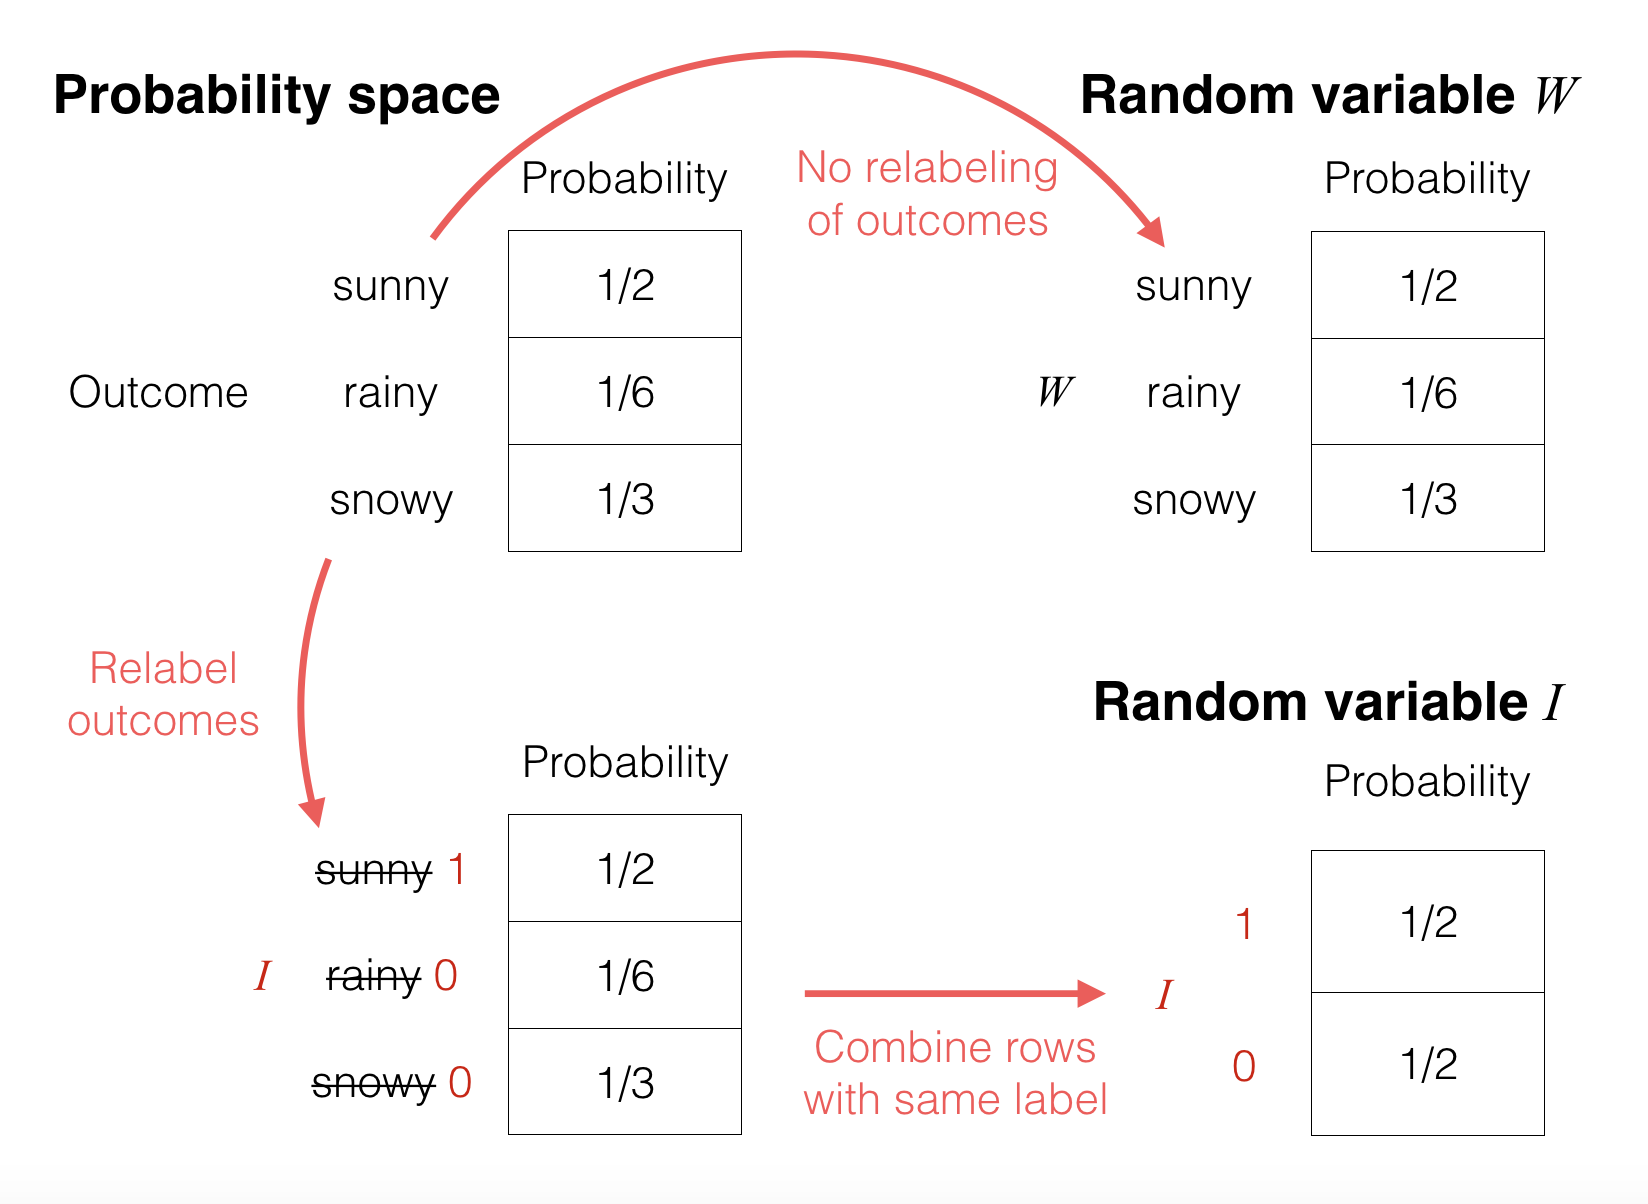
\includegraphics[scale=0.4]{images_sec-random-variables-main} \par}

These tables make it clear that a ``random variable'' really is just reassigning/relabeling what the values are for the possible outcomes in the underlying probability space (given by the top left table):

\begin{itemize}
\item In the top right table, random variable $W$ does not do any sort of relabeling so its probability table looks the same as that of the underlying probability space.

\item In the bottom left table, the random variable $I$ relabels/reassigns ``sunny'' to 1, and both ``rainy'' and ``snowy'' to 0. Intuitively, since two of the rows now have the same label 0, it makes sense to just combine these two rows, adding their probabilities $\frac{1}{6}+\frac{1}{3}=\frac{1}{2}$. This results in the bottom right table.
\end{itemize}

\paragraph{Technical note:} Even though the formal definition of a finite random variable doesn't actually make use of the probability assignment $\mathbb {P}$, the probability assignment will become essential as soon as we talk about how probability works with random variables.

\subsection{Two Ways to Specify a Random Variable in Code}

Two ways we can fully represent a random variable on a computer are as follows.

\paragraph{Approach 1.} Go with the mathematical definition of a random variable. First, specify what the underlying probability space is:

\begin{lstlisting}
> prob_space = {'sunny': 1/2, 'rainy': 1/6, 'snowy': 1/3}
\end{lstlisting}

Then provide a way to map from the sample space to the alphabet:

\begin{lstlisting}
> W_mapping = {'sunny': 'sunny', 'rainy': 'rainy', 'snowy': 'snowy'}
> I_mapping = {'sunny': 1, 'rainy': 0, 'snowy': 0}
\end{lstlisting}

Then we can generate a random sample/draw for random variables W and I:

\begin{lstlisting}
> random_outcome = comp_prob_inference.sample_from_finite_probability_space(prob_space)
> W = W_mapping[random_outcome]
> I = I_mapping[random_outcome]
\end{lstlisting}

\paragraph{Approach 2.} Remember how we wrote out probability tables for random variables W and I? Let's directly store these probability tables:

\begin{lstlisting}
> W_table = {'sunny': 1/2, 'rainy': 1/6, 'snowy': 1/3}
> I_table = {0: 1/2, 1: 1/2}
\end{lstlisting}

Treating the tables as probability spaces, draw samples for W and I:

\begin{lstlisting}
> W = comp_prob_inference.sample_from_finite_probability_space(W_table)
> I = comp_prob_inference.sample_from_finite_probability_space(I_table)
\end{lstlisting}


\subsection{Random Variables Notation and Terminology}

In this course, we denote random variables with capital/uppercase letters, such as $X$, $W$, $I$, etc. We use the phrases ``probability table'', ``probability mass function'' (abbreviated as PMF), and ``probability distribution'' (often simply called a distribution) to mean the same thing, and in particular we denote the probability table for $X$ to be $p_ X$ or $p_ X(\cdot )$).

We write $p_ X(x)$ to denote the entry of the probability table that has label $x \in \mathcal{X}$ where $\mathcal{X}$ is the set of values that random variable $\mathcal{X}$ takes on. Note that we use lowercase letters like $x$ to denote variables storing nonrandom values. We can also look up values in a probability table using specific outcomes, e.g., from earlier, we have $p_ W(\text {rainy}) = 1/6$ and $p_ I(1)=1/2$.

Note that we use the same notation as in math where a function $f$ might also be written as $f(\cdot )$ to explicitly indicate that it is the function of one variable. Both $f$ and $f(\cdot )$ refer to a function whereas $f(x)$ refers to the value of the function $f$ evaluated at the point $x$.

As an example of how to use all this notation, recall that a probability table consists of nonnegative entries that add up to 1. In fact, each of the entries is at most 1 (otherwise the numbers would add to more than 1). For a random variable $X$ taking on values in $\mathcal{X}$, we can write out these constraints as:

{\centering$0 \le p_ X(x) \le 1\quad \text {for all }x\in \mathcal{X}, \qquad \sum _{x \in \mathcal{X}} p_ X(x) = 1.$ \par}
 
Often in the course, if we are making statements about all possible outcomes of $X$, we will omit writing out the alphabet $\mathcal{X}$ explicitly. For example, instead of the above, we might write the following equivalent statement:

{\centering$0 \le p_ X(x) \le 1\quad \text {for all }x, \qquad \sum _ x p_ X(x) = 1.$ \par}


\end{document}